\documentclass{standalone}

\usepackage{tikz}
\usetikzlibrary{arrows.meta}

\begin{document}
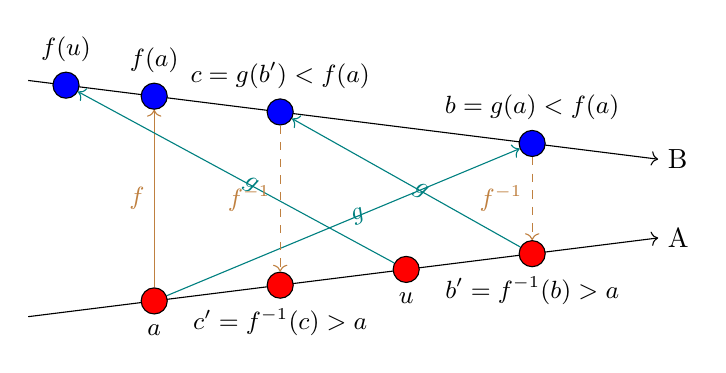
\begin{tikzpicture}[dot/.style 2 args = {pos = #1, draw, circle, fill = #2},
	every arrow/.style = {>=Stealth, ->}, font = \small]
	\draw[->] (0,0) to 
		node (a) [dot = {0.2}{red}, label = {below:$a$}] {} 
		node (c') [dot = {0.4}{red}, label = {below:$c' = f^{-1}(c) > a$}] {} 
		node (u) [dot = {0.6}{red}, label = {below:$u$}] {} 
		node (b') [dot = {0.8}{red}, label = {below:$b' = f^{-1}(b) > a$}] {}
			(8,1) node[right] {\normalsize A};

	\draw[->] (0,3) to 
		node (fu) [dot = {0.06}{blue}, label = {above:$f(u)$}] {} 
		node (fa) [dot = {0.2}{blue}, label = {above:$f(a)$}] {} 
		node (c) [dot = {0.4}{blue}, label = {above:$c = g(b') < f(a)$}] {} 
		node (b) [dot = {0.8}{blue}, label = {above:$b = g(a) < f(a)$}] {}
			(8,2) node[right] {\normalsize B};

	\draw[->, brown] (a) to node[left] {$f$} (fa);
	\draw[->, teal] (a) to node[sloped, right] {$g$} (b);
	\draw[->, teal] (b') to node[sloped, right] {$g$} (c);
	\draw[->, teal] (u) to node[sloped, right] {$g$} (fu);

	\draw[->, brown, dashed] (b) to node[left] {$f^{-1}$} (b');
	\draw[->, brown, dashed] (c) to node[left] {$f^{-1}$} (c');
\end{tikzpicture}
\end{document}